\section{Episode Restoration and Computational Cost}
\label{sec:closure-results}

Restoration timing gives a second view of continuous attribution. Figure~\ref{fig:closure-restoration} shows the signed OFF delay among available associated restorations, alongside intended events without a restoration value. Under the posthoc threshold of more than one 30-Hz report early ($d_{\rm OFF}<-1/30$ s), the physical bank has 0/644 early restorations and the nominal bank 0/643. The reference and short-window ExtraTrees have 52/330 and 26/352, respectively. The corresponding missing-restoration counts are 4, 5, 318 and 296 out of 648 intended event realizations. Missing values include omissions and are not necessarily open episodes. Replays are dependent; this descriptive criterion is not a new confirmatory endpoint and does not isolate the memory component.

\begin{figure}[t]\centering
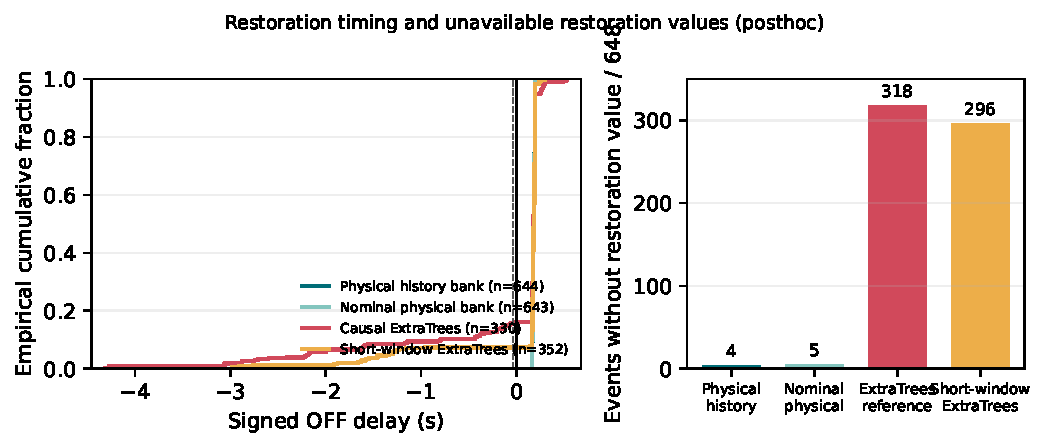
\includegraphics[width=\columnwidth]{figures/generated/closure_restoration.pdf}
\caption{Posthoc restoration timing and events without an associated restoration value. Panel A shows signed OFF delay only where available; the dashed line marks the threshold at one report early. Panel B reports missing restoration values over 648 intended events, including omissions, not a count of episodes open at record end.}
\label{fig:closure-restoration}\end{figure}

Recorded stage timings from the continuous evaluation are summarized in Table~\ref{tab:closure-compute-cost}. For 120-s records, median physical-history inference took 358.7 s across 270 records, compared with 9.5 s for the combined ExtraTrees adapter stage; physical bank construction had a separate 80.1-s median. Dividing total time by 3,601 reports gives amortized averages of 99.6 ms/report for physical inference and 2.6 ms/report for the combined learned stage. These totals include full-record work and do not measure per-report latency. The physical stage is slower in this recorded implementation and does not support a real-time claim. Timers span mixed stages from the evaluation and concurrency; memory use and frame-level latency were not recorded. The 600-s normal controls are summarized separately in the machine-readable cost file.

\begin{table}[t]\centering\footnotesize\setlength{\tabcolsep}{2pt}
\caption{Posthoc description of episode restoration in the continuous evaluation. Early counts restorations with $d_{\mathrm{OFF}}<-1/30$ s (more than one report early); Early (\%) divides by Available. Missing counts absent restoration values out of 648 intended events, including omissions and not necessarily open episodes. Replays are dependent; no significance test is implied.}
\label{tab:closure-restoration}
\begin{tabular}{@{}lrrrr@{}}\toprule
Method & Available & Early & Missing & Early (\%) \\\midrule
Physical bank & 644 & 0 & 4 & 0.0\% \\
Nominal bank & 643 & 0 & 5 & 0.0\% \\
ExtraTrees reference & 330 & 52 & 318 & 15.8\% \\
ExtraTrees short & 352 & 26 & 296 & 7.4\% \\
\bottomrule\end{tabular}\end{table}

\begin{table}[t]\centering\small\setlength{\tabcolsep}{3pt}
\caption{Recorded stage times from the continuous evaluation on 120-s records. Medians and ranges summarize full-record stages; the per-report column is a median-total divided by 3,601 reports and is amortized, not frame latency. Stages were recorded in a campaign with one BLAS and one Julia thread; memory and per-report latency were not recorded. This descriptive table does not establish real-time operation or a speedup under matched implementation conditions.}
\label{tab:closure-compute-cost}
\begin{tabular}{@{}lrrr@{}}\toprule
Stage & Median (s) & Range (s) & ms/report$^\dagger$ \\\midrule
Bank build & 80.1 & 62.0--309.7 & 22.2 \\
History inference & 358.7 & 218.2--2641.1 & 99.6 \\
ExtraTrees (both) & 9.5 & 6.7--50.5 & 2.6 \\
Chen detector & 1.3 & 0.9--10.6 & 0.4 \\
\bottomrule\end{tabular}\end{table}

